\documentclass[10pt,a4paper]{book}
\usepackage[utf8]{inputenc}
\usepackage{amsmath}
\usepackage{amsfonts}
\usepackage{amssymb}
\usepackage{makeidx}
\usepackage{graphicx}
\usepackage{hyperref}
\author{Marco Ricci}
\title{Appunti Ingegneria del Software}
\begin{document}
\tableofcontents
\newpage
\chapter{L'ingegneria del software e sviluppo agile}
\section{Software Engineering}
\paragraph{Definition IEEE} Software Engineering is the application of a systematic, disciplined, quantifiable approach to the development, operation, and maintenance of software; that is, the application of engineering to software.

\subsection{Software development activities}
...da fare

\subsection{Recent developments}
\begin{itemize}
\item Success of Open Source Software
\item Shift from producing software to using software
\item Software development becomes more heterogeneous
\item Rise of agile methods
\end{itemize}

\subsubsection{Open Source}
Perché si è diffuso enormemente il sw open source? Perché quando si sviluppa un software, se possibile si evita di reinventare la ruota ogni volta, utilizzando componenti, librerie, sorgenti e snippets di codice pronti all'uso.
Altro aspetto importante che ha contribuito al crescere dell'open source sono i motori di ricerca di codice.

\paragraph{Software ecosystems} Spesso si realizzano sistemi software composti da varie API di terze parti andando incontro a problemi relativi alle dipendenze, alle license, all'evoluzione delle componenti di terze parti.

\subsubsection{Shift from producing software to using software}
Paradigmi:
\begin{itemize}
\item Builders build pieces, integrators integrate them
\item Component-Based Development (CBSD)
\item Commercial Off-The-Shelves (COTS): componenti pronte all'uso, di ambito industriale
\item Software Product Lines (SPL): windows che ha varie versioni: pro, web, home
\item Service Orientation (SOA)
\end{itemize}

\subsubsection{Perché CBSE?}
Si sviluppa a componenti per aumentare la qualità, specialmente l'evolvibilità e manutenibilità. Inoltre aumenta la produttività e diminuiscono i tempi di sviluppo.

Tipicamente un componente implementa una funzionalità ed espone un'interfaccia (e.g. FACADE).
Lo sviluppo del componente avviene in maniera separata dallo sviluppo del sistema, ma entrambi hanno bisogno di un assessment (accertamento) che valuti il funzionamento del componente prima e dopo essere inserito nel sistema.

\subsubsection{Servizio}
Entità computazionale platform-indipendent richiamabile e accessibile tramite lo scambio di messaggi ad esempio col paradigma REST.
Aspetto importante dei servizi è che non vanno ospitati sulla macchina dell'utente perché vengono ospitati da altri host. Inoltre non bisogna tener traccia delle versioni in quanto questi saranno aggiornati lato server.

\subsubsection{Service lifecycle}
\paragraph{Analisi} basata sulla disponibilità dei servizi, progetto in base ai servizi disponibili.
\paragraph{Design} orchestrazione dei servizi.
\paragraph{Testing} testare i servizi e verificare periodicamente che essi non siano cambiati intaccando le funzionalità del sistema. Testare inoltre che il sistema sw rispetti determinati requisiti QoS.

Molti sistemi software che usiamo si basano su architetture orientate ai servizi: le app si affidano a servizi online per fornire le loro funzioni (ad esempio mappe, Facebook, Twitter, previsioni del tempo, app di prenotazione online, tabelle treni, stato dei voli).
I grandi sistemi software usano n-tier architetture che comunicano tra loro attraverso servizi.

\subsubsection{Servizio vs Componente}
Un servizio è più dinamico, QoS rilevante per la scelta dei servizi, mancanza di controllo sul servizio che si sta usando

\subsection{App stores}
Altro cambiamento forte nello sviluppo software è quello del suo rilascio mediante gli store, a differenza di qualche anno fa quando questo veniva distribuito via CD/DVD.
Esempi di store sono iOS App Store, Google Play, Playstation network store, Steam, ecc.
Gli store permettono aggiornamenti frequenti a differenza del passato quando la versione distribuita doveva essere stabile per evitare aggiornamenti problematici data la modalità di distribuzione.
Oggi invece andare sul mercato prima della concorrenza è più importante che rilasciare un prodotto di qualità.
Gli store hanno inoltre introdotto le recensioni e i rating per il software. Le recensioni degli utenti rappresentano una fonte importante per il crowdsourcing dei requisiti.
Tuttavia per app con milioni di recensioni diventa impossibile leggerle tutte, ci saranno recensioni inutili e duplicate. Per venire incontro all'esigenza di filtrare le recensioni nascono dei tool che le raggruppano per argomento, per versione del software o le fattorizzano secondo altri parametri.

\section{Agile Methods}
\textbf{Perché Agile?} Per produrre software è richiesta un bel po' di documentazione, i requisiti cambiano molto nel tempo \textbf{(requisiti non stabili)}, le tecnologie e i tipi di software cambiano velocemente nel tempo (nuovi linguaggi, nuovi dbms...). Quindi lo sviluppo software convenzionale non va più bene, o meglio, diventa molto più difficile e articolato (valle di lacrime Larry).

Questo è il modello a cascata. Esso è molto pesante poiché bisogna "congelare" i requisiti prima di passare al design e così via.\\\\
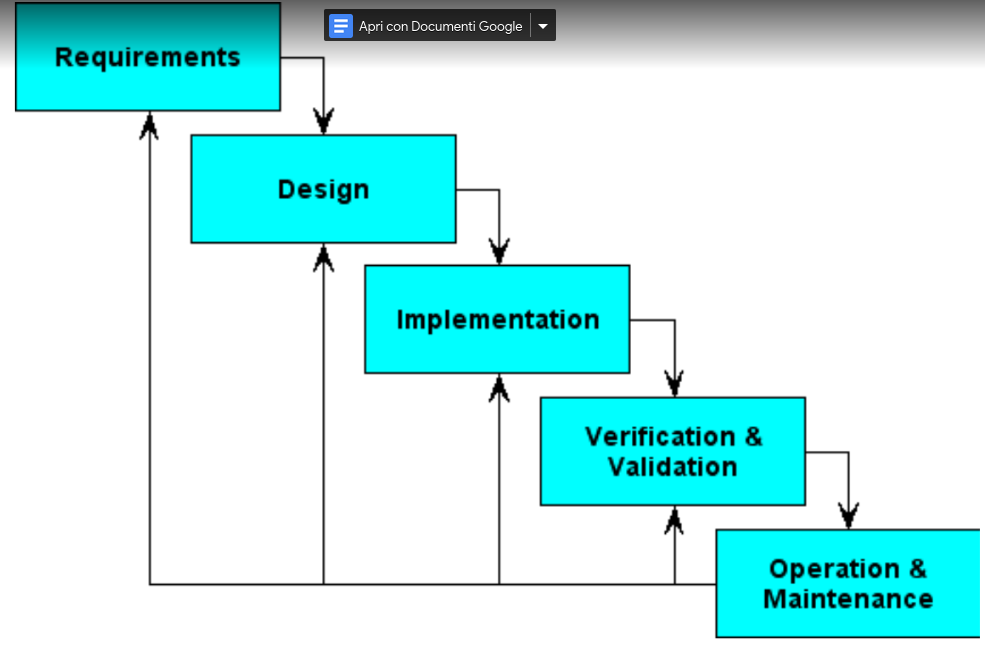
\includegraphics[scale=0.2]{waterfall.png}\\

Successivamente è stato concepito il modello a spirale il quale funziona tramite iterazioni di passaggi: determinazione obiettivi, risolvere problemi, sviluppo e test, nuova iterazione.\\\\
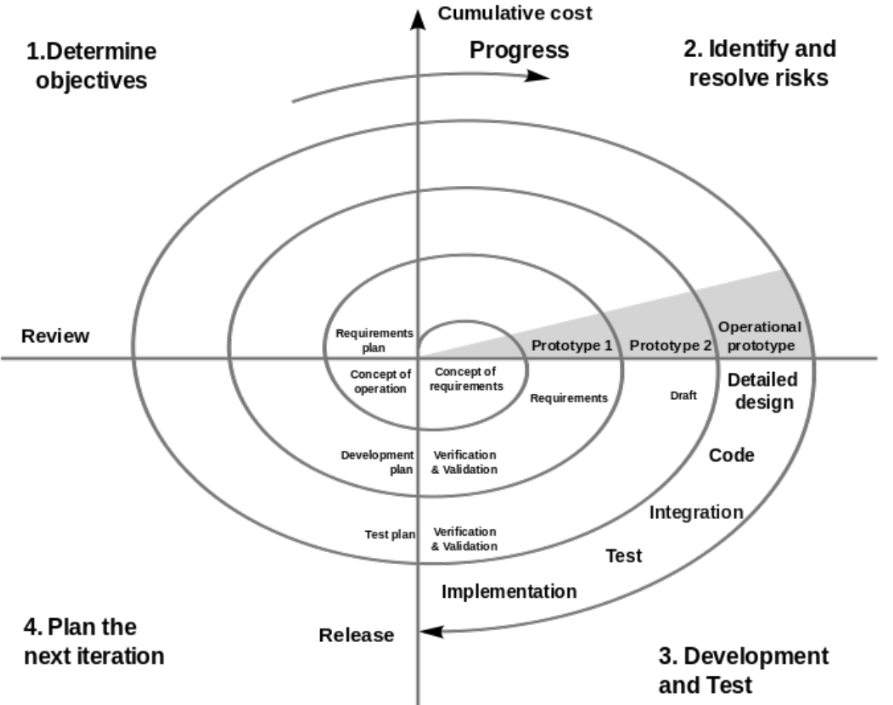
\includegraphics[scale=0.2]{spiral.png}\\

Il modello Agile è un'estremizzazione del modello a spirale, composto da tante spirali.\\\\
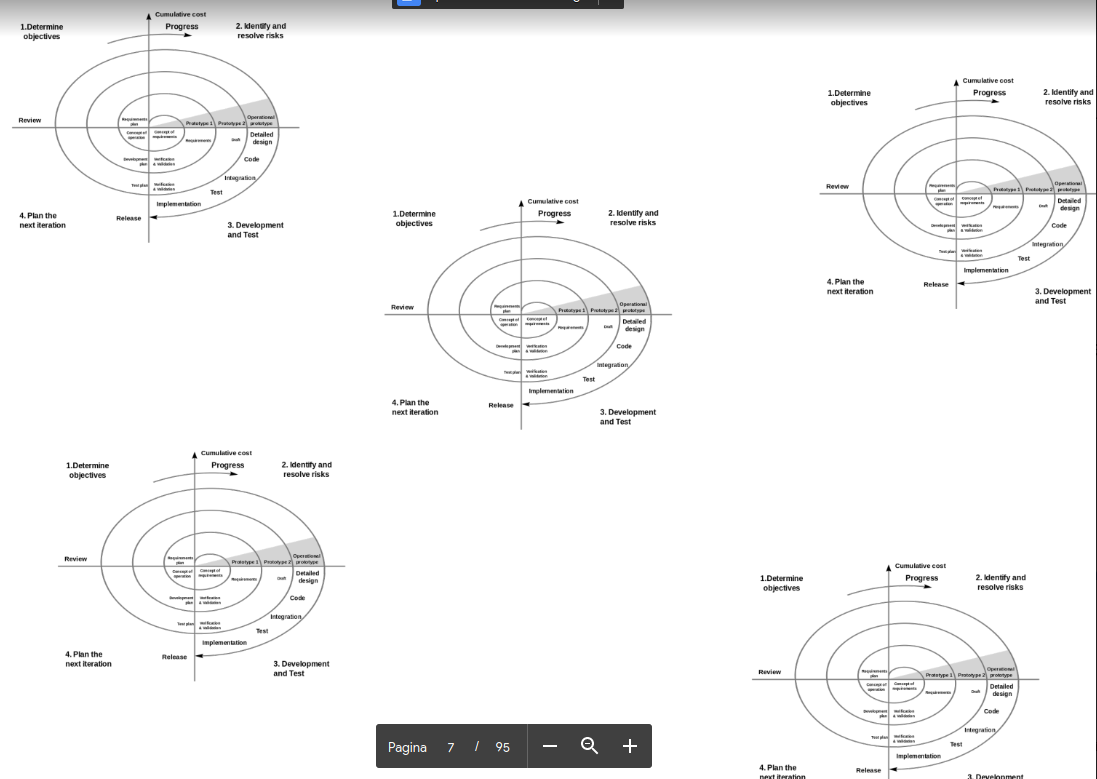
\includegraphics[scale=0.2]{agile.png}\\

\subsection{The Agile Manifesto}
Punti cardine di Agile:
\begin{itemize}
\item Fare in modo che ci sia una corretta comunicazione tra gli individui, ogni membro del team sa delle decisioni prese e dell'andamento generale dello sviluppo
\item Ad ogni push bisogna avere un programma funzionante (e.g. se entra il capo o il committente bisogna essere in grado di dimostrare il funzionamento del software)
\item Continua collaborazione col committente a fronte di cambiamenti dei requisiti ecc. Scrivi requisiti in maniera leggera, agile, per consentirne eventuale rinegoziazione.
\item Non si segue un piano rigido, ma si cerca di rispondere ai cambiamenti
\end{itemize}

\subsection{Extreme Programming}
In Agile ci sono diverse pratiche. Una delle prime più diffuse è quella \textbf{Extreme Programming} sviluppata da Kent Beck. 
Tipicamente utilizzata in piccole organizzazioni, la sua idea è porre molta attenzione sulla comunicazione tra sviluppatori, avere continui feedback, ma soprattutto avere release continue e frequenti.
Pratiche adottate in EP sono sviluppo test-driven e continuous refactoring (applicare modifiche al codice per migliorarne leggibilità, manutenibilità, performance).

\subsection{Scrum}
Altra pratica è quella di Scrum, simile a XP perché si sposa bene a un cambiamento veloce di requisiti.
Rispetto a XP, SCRUM prevede un po' più di rigidità, infatti si pone tra XP, che è più anarchica, con rilasci veloci, e i processi di sviluppo tradizionali in cui i rilasci sono schedulati ogni tot mesi.
Prevede iterazioni più lunghe (sprint lunghe non meno di 15 giorni).

Scrum prevede, all'interno di un progetto, diversi \textbf{ruoli}, \textbf{cerimonie}, che sono una serie di attività (planning sprint, sprint review..), \textbf{artifact}

\subsubsection{Ruoli Scrum}
\paragraph{Product Owner} Chi è? O chi paga o il manager di azienda. Su cosa ha voce? Sul budget, sui tempi, scadenze, prioritizzazione.

\paragraph{Scrum Master} Tipicamente il team leader, che si assicura che la metodologia Scrum è applicata correttamente, ma soprattutto è la persona che guida gli stand-up meeting, \textbf{capisce se ci sono problemi e cerca di risolverli} (problemi di natura tecnica ma anche umana), mantiene alta la produttività.

\paragraph{Project Team} L'aspetto principale del Team Scrum è la dimensione ridotta, tipicamente composto da 5-10 membri. Inoltre essi sono Cross-functional, ovvero ogni team non è specializzato in un ambito, ma deve avere tutte le espertistiche (figure come programmatori, designer, tester...) che servono almeno per la sprint su cui lavorano. Quindi i team di design, programmatori, tester non sono separati tra loro, ma ogni team possiede almeno una figura di ognuno.

%lez 2021-09-28
\subsubsection{Pianificazione progetto Scrum}
Un progetto Scrum viene pianificato scrivendo delle User Stories, pianificando le release, dividendolo in più iterazioni applicando il modello a spirale ma ripetuto frequentemente, fare una volta al giorno lo stand up meeting.

Le iterazioni il progetto viene diviso in base al piano di rilascio, vengono considerati rilasci brevi ma distinti (tipicamente una sprint o due al mese)

\paragraph{Product Backlog} lista di requisiti. Pila di post-it che specifica i requisiti del progetto
Team capacity: dimensione e numero di team.
Condizioni di business: scadenze, budget.
Tecnologia: tecnologia utilizzata

\paragraph{Daily scrum meeting} brevi incontri da fare in mattinata, velocemente (15 min), stand up, definire cosa fare durante il giorno e capire se ci sono problemi.
Normalmente partecipano anche lo scrum master e il product owner oltre ai membri del team.

\paragraph{Scrum's Artifact} product backlog (user story), spring backlog (sottoinsieme di user stories assegnato a una certa spring), burndown charts (una sorta di progress bar che ci indica l'avanzamento del processo produttivo).

\paragraph{Product Backlog} requisiti, lista di user stories applicate alla sprint, stimate per difficoltà di realizzazione.

\paragraph{Tipi di requisiti} 
per richiedere nuove funzionalità o cambio di funzionalità preesistenti.
associati a un bug
task tecnologici
investigazioni relative a tecnologie che voglio utilizzare per cercare di capire se quella tecnologia può essere utile e quindi adottata

\paragraph{User Stories} scritte dai customers in linguaggio naturale, simili ai casi d'uso, ma scritte diversamente (il caso d'uso descrive l'interazione tra l'attore è il sistema, e non una commutazione interna). Idealmente possono essere utilizzate per generare casi di test di accettazione, mentre sviluppo monitoro il progresso dello sviluppo della userstory eseguendo casi di test (da vedere in pratica con i tool).

\paragraph{Com'è scritta una user story?} Specificando il who (l'attore, user role), il what (goal,obiettivo), il why (reason, perchè raggiungere l'obiettivo).

\paragraph{Struttura tipica} As a [user role], I want to [goal], so I can [reason].

\textbf{Example}: "As a user, I want to log in, so I can access subscriber content."

\paragraph{Story Points} stima, assegnata alla user story, che indica lo sforzo necessario per implementare la storia.
la stima è rappresentata da scale, le più comuni sono: 1-10, t-shirt size (XS, S,M,L,XL), serie di Fibonacci. Ogni scala ha una 'grana' più fine o più grossolana, il quale utilizzo viene adattato alla complessità della storia in esame.
 
\paragraph{Features} l'unità più piccola di requisito da realizzare in un sistema consiste in una user story. 
Scrum definisce dei livelli più alti di aggregazione delle user stories, il primo livello è quello delle features, un pezzo di funzionalità completo da rilasciare nel mio sistema. Simile a una user story, ma composto da più user story. Testabile. Mentre le user stories sono spesso assegnate a una sprint, le features possono spalmarsi su più sprint.

\textbf{Esempio}.....



\paragraph{Epica} più grande della feature, rappresenta un macrogoal del progetto, quindi una direzione. Riguarda più sprint, ma può riguardare anche più release pubbliche. Molto spesso l'epica potrebbe avere a che fare con grosse decisioni strategiche relative al prodotto che potrebbero portare alla scelta del prodotto rispetto ad un altro concorrente.

\textbf{Esempio}: disponibilità dati sul traffico, importante perché può influenzare diverse caratteristiche del prodotto come il reindirizzamento o il calcolo del percorso corrente;
ancora, gestire o meno i danni sulle auto in un gioco di simulazione automobilistico il che può influenzare la fisica delle corse, il pit stop dell'auto per la riparazione, ecc.

Epica > feature > user story

\paragraph{Temi} livello più alto delle epiche, non sempre necessario, sono sostanzialmente obiettivi di progetto.




\subsection{Design in agile}
Semplice, minimale, serve a chiarire le idee. 
Refactor quando possibile

\textbf{CRC Card}: descrivono per ciascun pezzo di funzionalità quali sono le azioni e le info di cui deve tenere traccia.

\subsection{Coding}
Bisogna utilizzare standard condivisi di codice(nome classi, nome variabili,...) in quanto il codice è la più aggiornata forma di documentazione del progetto e deve essere conosciuto da tutti.
Pair Programming: due persone che lavorano insieme, davanti lo stesso monitor, uno scrive il codice ee l'altro fa code review on the fly, o fa supporto, o dà suggerimenti sulle api da usare. Poi ci si scambia di ruolo.
Collettive code ownership: Tutti devono conoscere il codice di tutti.
I casi di test tipicamente sono scritti prima del codice
integrazione prima possibile, avere un working project  (continuous integration) progetto sempre funzionante 
avere prima un progetto funzionante, poi ottimizzare. da non fraintendere con un arronzamento totale.

\subsection{Testing}
Casi di test scritti prima del codice. Perché utile? serve da guida per capire ciò che si sta implementando.

casi di test di accettazione sono derivati dai requisiti e quindi di alto livello, relativi all'interno sistema, scritti tipicamente col cliente.
casi di test di unità relativi a una singola funzionalità/unità/classe/funzione derivati dalla specifica della funzionalità, a livello di api.


Essenza di Agile
Test first dove possibile, ridocumentare durante lo sviluppo, avere casi di test di accettazione che guidano durante lo sviluppo ed effettuare refactoring continuo.



ultimi 20 minuti lez 2021-09-28 09-04-58 : pratica icescrum, slack(discord)

user stories -> backlog di progetto -> backlog viene pianificato allocando le user stories su delle spring (scadenze interne mensile o 15 giorni) -> progress stimato dalla complessità della story -> story point -> uso grafici per montorare i progressi di quanto è implementato o resta da implementare

\newpage
\chapter{Software configuration management SCM}
\textbf{Scenario}: più persone che lavorano su un sistema software soggetto a cambiamenti e si ha la necessità di supportare più versioni di questo sistema: più sistemi rilasciati, parte di sistema sotto sviluppo...
C'è bisogno di coordinazione tra gli sviluppatori, gestire l'evoluzione dei sistemi software e controllare i costi e i rischi relativi ai cambiamenti effettuati nel sistema.

\textbf{Definizione}: insieme di attività che disciplinano all'interno di un processo di ingegneria del software ciò che è necessario a sviluppare una baseline, una sorta di snapshot di un sistema software che ha determinate caratteristiche. Quindi SCM è un qualcosa che disciplina lo sviluppo di sw in un ambiente cooperativo.

\textbf{Descrizione}: SCM si occupa di disciplinare il processo di iniziazione di una repository sw, valutare e controllare i cambiamenti durante e dopo il processo di ingegnerizzazione.

Stanadrd IEEE 828 da usare come template per redigere il piano.

SCM è una funzione del progetto (come definito nel SPMP) con l'obiettivo di rendere le attività tecniche e manageriali più efficaci.
La gestione della configurazione del software può essere amministrata in diversi modi:
\begin{itemize}
\item Un unico team di gestione della configurazione del software per intera organizzazione
\item Un team di gestione della configurazione separato per ogni progetto
\item Gestione della configurazione del software distribuita tra i membri del progetto
\item Miscela di tutti i precedenti
\end{itemize}

\section{SCM activities}
\begin{itemize}
\item Configuration item identification: capire quali sono gli artefatti da mettere sotto controllo e configurazione.
\item Promotion management: quali sono condizioni e requisiti per rilasciare codice agli altri sviluppatori.
\item Release management: quali sono requisiti che un pezzo di codice/software deve rispettare affinché possa essere rilasciato.
\item Change management: la gestione, l'approvazione e il monitoraggio di richieste di modifica.
\item Branch management: gestione di creazioni di sviluppi concorrenti.
\item Variant management: gestione delle varianti nel caso di software
\end{itemize}

Tutte queste attività possono essere gestite senza avere in mente delle regole ben definite. Può esserci gestione formale o informale e molto dipende dal progetto.

\subsection{Configuration management roles}
\begin{itemize}
\item Configuration Manager: responsabile di identificare gli \textbf{item di configurazione}.
\item Change control board member: responsabile di approvare le change request.
\item Developer: sviluppatore.
\item Auditor: responsabile della selezione e della valutazione delle promozioni per il rilascio e per assicurare la coerenza e la completezza di questo rilascio
\end{itemize}


\subsection{CM Tools}
\begin{itemize}
\item Version Control: CVS, Git,..
\item Bug (issue) tracking, bugzilla..
\item Build ant, maven, gradle.
\item Project management: sourceforge.net, freshmeat.net, gforge...(non ce ne occuperemo)

\end{itemize}

\subsection{Configuration Item} è un artefatto sia HW che SW per il quale si deve mantenere nel sistema di configuration management un controllo di versione. Significa non solo mantenere traccia della versione di tale artefatto, ma anche sapere in ogni versione del sistema software rilasciata all'esterno quale versione di una data componente(e.g. base di dati, algoritmo per un qualcosa ...) è al suo interno.

Software configuration items are not only program code segments but all type of documents according to development, e.g.
!all type of code files
!drivers for tests
!analysis or design documents
!user or developer manuals
!system configurations (e.g. version of compiler used)

In some systems, not only software but also hardware configuration items (CPUs, bus speed frequencies) exist! (e.g. arduino, sensori, cpu, ecc)

\subsubsection{I passo: definire i configuration item}

Quando si lavora con progetti molto grandi vengono prodotte entità(file, documenti, data,..) che vanno identificati univocamente.
Qualsiasi entità del processo di ingegneria del software può essere sotto configuration management control, ma non tutte le entità lo necessitano per tutto il tempo.
Quindi va analizzato \textit{cosa} diventa un configuration item e se mettere sotto controllo\\
e anche \textbf{quando} tale entità va messa sotto configuration control.
Iniziare troppo presto con la CI introduce troppa burocrazia, mentre iniziare troppo tardi introdurrà caos nel progetto.

\paragraph{Evitare repository 'gonfi'}
Componenti di terze parti come librerie, dipendenze ecc possono non essere caricate nel repository del progetto in quanto ci sono i tool di build automation (maven, gradle) che li scaricano automaticamente on the fly dalla rete.

Tuttavia, bisogna anche fare attenzione alla compilabilità a lungo termine del progetto poiché tra un po' di tempo tali dipendenze potrebbero non essere più disponibili.

Una volta che i Configuration Item sono selezionati, di solito vengono organizzati in una struttura ad albero (ramo dei modelli, dei documenti, del codice...).

\subsection{Terminologia: Versione}
La versione è un rilascio di un progetto verso l'esterno. Diverse versioni hanno diverse funzionalità.

\subsection{Terminologia: Baseline}
Lo stato di un prodotto che è stato definito in maniera formale dal management di configurazione.
e.g. Baseline A:Punto dell'evoluzione del progetto in cui sono definite tutte le API.
	Baseline B: GUI implementata.
	
Man mano che i sistemi vengono sviluppati, viene sviluppata una serie di baseline, di solito dopo una
revisione (revisione dell'analisi, revisione del progetto, revisione del codice, test del sistema, accettazione, ...)

In uno sviluppo tradizionale si potranno avere delle baseline in cui è pronto il design o i requisiti o rilascio di un prototipo, alpha, beta, ecc.
Per quanto riguarda un processo di sviluppo SCRUM tutti gli esempi visti su vanno a collidere all'interno di una sprint.\\
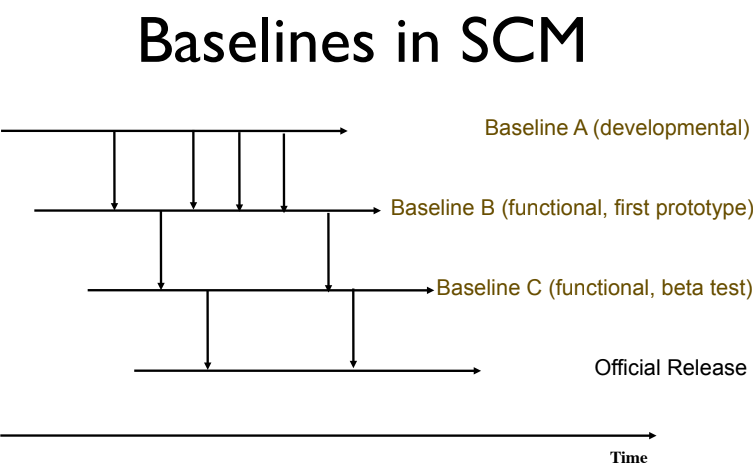
\includegraphics[scale=0.45]{baseline.png} 

\subsection{Versione, variante, revisione}
\textbf{Versione}: un CI a un certo punto del suo sviluppo, include la revisione e variante. (e.g. la versione 1.3 è vista come la revisione della 1.2)
\textbf{Revisione}: è una versione in una catena di modifiche.
\textbf{Variante}: versioni con funzionalità equivalenti(non sempre), ma sviluppate per impostazioni diverse (hardware e software).
\textbf{Branch}: ramo, sequenza di versioni nella timeline.

Come si indicano le versioni di un CI?
Il più popolare è quello basato su tre cifre: \begin{verbatim}<version>::=<configuration item name><major><minor><revision> \end{verbatim}

Major: cambia quando c'è rivoluzione nel sistema.
Minor: cambia con l'aggiunta di piccole funzionalità.
Revision: bugfix.\\
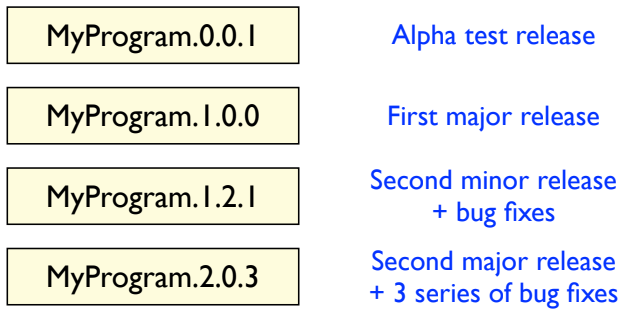
\includegraphics[scale=0.45]{version.png} 

Con il branch invece si va ad aggiungere un numero in più. (e.g. 1.2.1.1)

\paragraph{Altro schema di numerazione}
a.b.c.d\\
-a - major (delivered)\\
-b - minor (delivered)\\
-c - revision (internal)\\
-d - build (incremented by the continuous integration process)\\

\newpage
\section{Change management}
\marginpar{videolezione 2021-10-04}
\`{E} la gestione delle richieste di cambiamento. Regole da seguire quando qualcuno, sia all'interno del progetto sia all'esterno, richiede di effettuare un cambiamento. e.g. bugfix, richiesta di nuova feature..
Processo generale: richiesta di cambiamento, se il cambiamento viene accettato viene assegnato a qualcuno, viene implementato, viene verificato(review, testing).
La gestione dei cambiamenti può essere più o meno strutturata, in base alla complessità del processo o del cambiamento stesso.

\subsection{Controlling changes}
\begin{itemize}
\item Promotion: 
\item Release: politiche da adottare per mettere il SW a disposizione degli utenti.\\
\end{itemize}
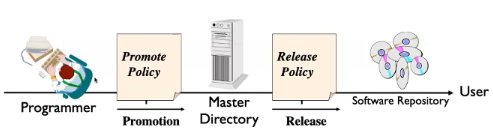
\includegraphics[scale=0.7]{changes.png} 

\subsubsection{SCM Directories}
Il software può trovarsi in tre punti: in locale(macchina del programmatore), master directory(repository centralizzato), software repository(punto in cui il software è a disposizione dell'utente).

\subsubsection{Change Policies}
Ogni volta che viene eseguita una promozione o un rilascio, una o più politiche si applicano. Lo scopo delle politiche di cambiamento è di garantire che ogni versione, revisione o rilascio (vedere la prossima diapositiva) sia conforme a criteri comunemente accettati.
Examples for change policies:\\
“No developer is allowed to promote source code which cannot be compiled without errors and warnings.”\\

“No baseline can be released without having been beta-tested by at least 500 external persons.”\\

\section{Software Configuration Management Plan}
Lo SCMP può seguire uno standard pubblico come l'IEEE 828, o uno standard interno (ad esempio specifico dell'azienda).

Cosa è importante definire in un SCM plan? quali sono gli artefatti da gestire?
\begin{itemize}
\item tipo di documenti da gestire e schema di nomenclature di essi(classi, variabili, versioni,...).
\item chi è responsabile per le procedure di CM.
\item politiche di cambiamento (viste prima)
\item tools da utilizzare nel CM process
\end{itemize}

\subsection{SCMP Section 1, intro}
\begin{enumerate}
\item Panoramica semplificata delle attività di CM.
\item scopi:
	\begin{itemize}
		\item descrizione panoramica del progetto
		\item identificazione dei CI a cui viene applicata la configuration management
	\end{itemize}
\item identificazione di altri software da includere come parte dello SCMP(SW di supporto, testing)
\item Ipotesi che potrebbero avere un impatto sul costo, sul calendario e sulla capacità di eseguire le attività SCM definite.
\item grado di formalità
\item limitazioni e vincoli di tempo per applicare l'SCM a questo progetto
\item Relazione di SCM con l'hardware della configurazione del sistema attività di gestione
\end{enumerate}
\subsection{SCMP Section 2, management}
\begin{itemize}
\item Organizzazione
\item Responsabilità
\item Politiche applicabili
\end{itemize}
\subsection{SCMP Section 3, acivities}
3.1 Configuration Identification\\
3.2 Configuration Control\\
3.3 Configuration Status Accounting\\
3.4 Configuration Audits and Reviews\\
3.5 Interface Control\\

\subsubsection{3.2 Configuration control}
Defines the following steps\\
3.2.1 How to identify the need for a change (layout of change request form)\\
3.2.2 Analysis and evaluation of a change request\\
3.2.3 Approval or disapproval of a request\\
3.2.4 Verification, implementation and release of a change\\

\subsubsection{3.2.1 Change request}
Specifica le procedure per richiedere una modifica a un baseline CI e le informazioni da documentare:
nomi e versioni del CI in cui appare il problema
originator's name and address
data richiesta
indicatore di urgenza
descrizione della richiesta di cambiamento

\subsubsection{3.2.2 Valutazione del cambiamento}
Specifica l'analisi richiesta per determinare l'impatto dei cambiamenti proposti e la procedura per la revisione dei risultati dell'analisi.

\paragraph{Gestire bug duplicati} Problema: Spesso vengono reportati bug che già erano stati segnalati e forse il bug è stato addirittura fixato.
Come riconoscerli? basarsi su similitudine testuale del report, ma anche utilizzare informazioni strutturali del report stesso esempio se è presente la stack trace confrontare anche quella.

\paragraph{Bug triaging} Dato un bugreport o una change request, a chi viene assegnata?
A chi in passato aveva fixato bug simili, anche su questo si esamina la similarità dei bug report.

\subsubsection{3.2.3 Approvazione o disapprovazione del cambiamento}
Questa sezione dello SCMP descrive l'organizzazione della scheda di controllo della configurazione (CCB).
CCB può essere un individuo o un gruppo, responsabile di approvare o no i cambiamenti.
Sono anche possibili più livelli di CCB, a seconda della complessità del progetto
Possono essere specificati più livelli di CCB. In piccoli sforzi di sviluppo un solo livello di CCB è sufficiente.

\subsubsection{3.2.4 Implementazione del cambiamento}

\subsubsection{3.3 Configuration Status Accounting}

\subsubsection{3.4 Configuration Audits and Reviews}

\subsection{Forma di un SCMP}
Lo SCMP può essere un documento separato o una sezione incorporata in un altro documento, per esempio nel SPMP, intitolato "Software Configuration Management Plan".
Informazioni minime da inserire: 6 sezioni: Introduzione, Gestione, Attività, Programmi, Risorse e Manutenzione del piano.\\

Criteri di coerenza (da usare in una riunione di revisione del SCMP):\\
- Tutte le attività definite nel SCMP (sezione da 3.1 a 3.6) sono assegnate a un'unità organizzativa o persona.\\
- Tutti gli item di configurazione identificati (Sezione 2.1) hanno processi definiti per la creazione di baseline  e controllo delle modifiche (sezione 3.2)\\
- Tutte le attività sono associate a risorse (sezione 5) per realizzare le attività.\\

\section{Code Review-> Software Inspection}
Una tecnica di analisi statica degli artefatti del sistema SW che si basa sull'esame visivo dei prodotti di sviluppo \textbf{per rilevare errori}, \textbf{violazioni degli standard di sviluppo} e altri problemi.
Prima avveniva fisicamente, si leggeva il codice ad un meeting. Ora avviene mediante strumenti automatici.
\paragraph{Cos'è?}
Esame sistematico del codice sorgente, spesso fatto per accettare o rifiutare una patch, finalizzato a:\\
- Trovare i bug\\
- Identificare l'uso scorretto del lessico / commenti scadenti\\
- Identificare scelte di design scadenti/stili di codifica scadenti\\
- Revisioni collaborative supportate da sistemi di versioning o da sistemi specifici come \textbf{gerrit}\\

\subsection{Development with/without Code Review: Gerrit}
Senza gerrit gli sviluppatori farebbero push direttamente nel repository centrale del progetto. Quindi la code review non interviene.\\
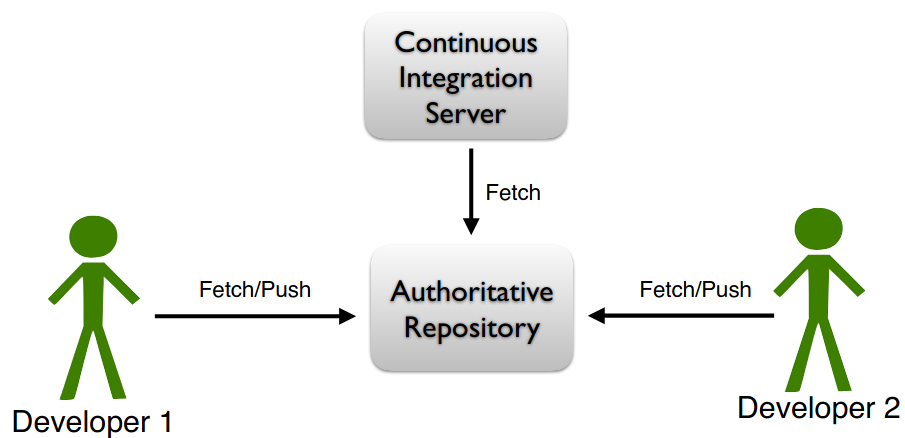
\includegraphics[scale=1]{nocoder.png} \\ \\

Con gerrit viene aggiunto un ulteriore repository(di pending changes) oltre al centrale.
Questo repository su gerrit ospiterà i push degli sviluppatori fin quando i revisori approvano i cambiamenti. Successivamentegerrit automaticamente effettua il merge del cambiamento e quindi il push sul repo centrale.\\
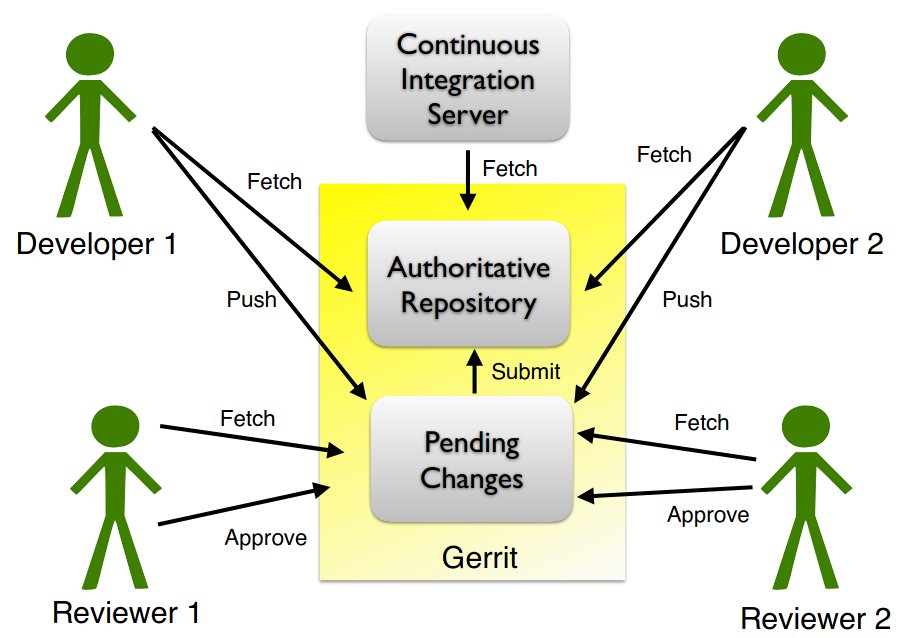
\includegraphics[scale=1]{coder.png} \\ \\

Alternative a gerrit sono le pull request di github e gitlab.

\subsection{Code Review, How?}
Cosa si fa durante un processo di code review? quali sono gli obiettivi?

Il processo può essere tenuto da individui singoli o da team. Importante è settare gli obiettivi, come le linee di codice da revisionare in un giorno.
Affinché il processo abbia senso bisogna usare una checklist. La checklist contiene una serie di aspetti che devono essere controllati:
\begin{itemize}
\item Wrong use of data: variable not initialized, dangling pointer, array index out of bounds, ...)
\item Faults in declarations: undeclared variable, variable declared twice, ...
\item Faults in computation: division by zero, mixed-type expressions, wrong operator priorities, ...
\item Faults in relational expressions: incorrect Boolean operator, wrong operator priorities, .
\item Faults in control flow: infinite loops, loops that execute n-1 or n+1 times instead of n, ..
\end{itemize}

Esempio di checklist su slide 92. 
Esempio studio code review di microsoft slide 97. Tool code flow. risultati raggiunti: articolo su drive

\begin{Large}textbf{setup tutorial di gerrithub}\end{Large} slide successive\marginpar{videolezione 2021-10-04}

il progetto si clona direttamente da gerrithub, ovviamente linkato con github, perché così ci si mette nell'ottica del revisore.
Download remote git hooks
push changes to gerrithub

i cambiamenti saranno visibili in gerrithub

\subsection{Can we automate code reviews?}
Automated code reviews: Nothing replace code reading but... Some problems can be pinpointed by automated tools\\
Examples of tools for Java: PMD, CheckStyle(verifica che il codice rispetti gli standard definiti, indentazione, parentesi, blocchi; configurazioni di stile in un file xml, alcune già pronte), FindBugs.\bigskip 

Esempio utilizzo dei tool di code review\marginpar{videolezione 2021-10-05}

\section{Promotion Release, Branch and Variant Management}
\subsection{Promotion Management}
Lo sviluppatore condivide le proprie configurazioni con gli altri.

\subsubsection{Promotion Requirements}

\subsubsection{Promotion Management: Discussion}



\subsection{Release Management}
Processo molto più accurato



\subsection{Branch Management}
Un branch si ha quando diversi team di sviluppo lavorano su diverse componenti in maniera concorrente, tenendo anche conto che tali linee parallele possono non ricongiungersi con la linea principale(master, main)(e.g. perché tale feature non serve più o non è valida, oppure potrebbero diventare nuovi prodotti).

Un branch tipicamente si apre quando un team vuole lavorare su una feature in maniera concorrente. \\
Esempio:\\

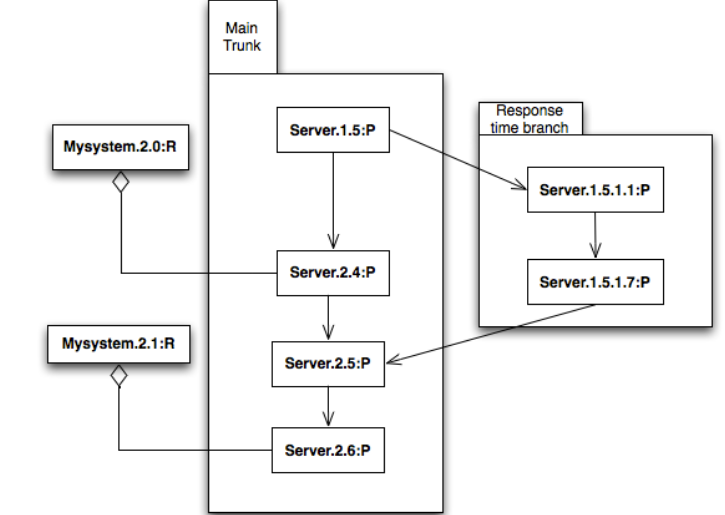
\includegraphics[scale=0.35]{branch.png} \\ \\

\subsubsection{Euristiche per il BM}
Si utilizzano euristiche per evitare problemi relativi al branch management
\begin{itemize}
\item capire subito quali sono i \textbf{punti di overlap}(sovrapposizione) per evitare conflitti tra i team di sviluppo paralleli
\item \textbf{Merge frequenti} per fare in modo che i team siano sempre sincronizzati e il codice aggiornato. (Più tempo passa prima del merge di un branch, più il branch diventa pericoloso e difficile da riunire col main)
\item Comunicazione: i team lavorano indipendentemente, ma devono comunicare per evitare e prevenire conflitti.
\item Minimizzare i cambiamenti nel main trunk per ridurre conflitti, quindi, meglio lasciare che lo sviluppatore faccia le modifiche nel branch.
\item minimizzare il numero dei branch
\end{itemize}


\subsection{Variant Management}
La gestione delle varianti si ha quando si va a sviluppare delle product line, varianti dello stesso sistema con funzionalità leggermente diverse destinate a diverse piattaforme SW o HW.
Come può funzionare la gestione di un progetto in varianti?
\begin{itemize}
\item Team ridondanti: ogni team ha la sua variante e la sua linea di sviluppo indipendente, poco codice condiviso.
\item Progetto singolo con una parte in comune e un'altra no che costituisce la variante.\\
\end{itemize}
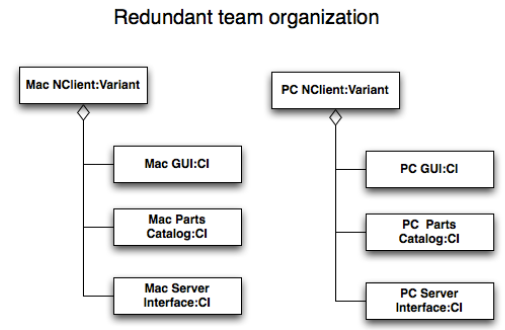
\includegraphics[scale=0.35]{redu.png} 
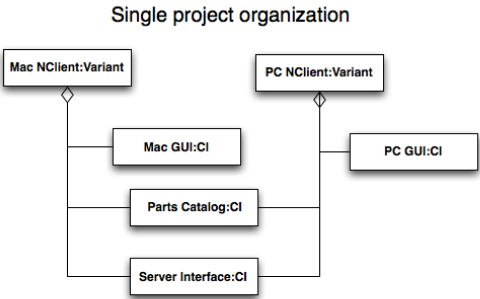
\includegraphics[scale=0.35]{single.png} \\ \\

\subsubsection{Issue dovuti alla condivisione di codice}
Problematiche legate alla seconda soluzione (code Sharing).
\paragraph{Single supplier/multiple customers}
Si possono avere delle core subsystem, parti in comune, usate da diversi team che lavorano su diverse varianti, anche con requisiti diversi.
Nasce quindi la necessità di fare un'attenta gestione del cambiamento per determinare se il cambiamento è specifico della variante o se riguarda l'intero sistema.
Se il cambiamento riguarda tutte le varianti, allora dovrebbe essere fatto sulla parte comune, non nelle varianti.

\paragraph{Long change request turnaround}
l'implementazione di un problema specifico di una variante può richiedere molto tempo perché il team deve verificare che non abbia impatto su altre varianti.
Soluzioni:
- coinvolgere il team che ha emesso la richiesta di cambiamento durante la convalida.
- il cambiamento è implementato, promosso e rilasciato solo alla variante da cui proviene la richiesta.
- dopo la convalida, altre varianti possono iniziare ad usare il sottosistema rivisto.

\paragraph{Cross-platform inconsistencies}
sottosistemi di base introducono vincoli sui sottosistemi specifici della variante sottosistemi\\
- ad esempio, sottosistemi di base con un flusso di controllo filettato, una l'interfaccia grafica di una variante è guidata dagli eventi\\
Soluzioni:\\
- anticipare la progettazione specifica della variante\\
- i sottosistemi principali dovrebbero concentrarsi su una variante indipendente decomposizione del sottosistema\\
- le incoerenze cross-platform di livello inferiore sono affrontate in sottosistemi specifici della variante\\

\subsection{Software Product Lines}
Come vengono gestite le linee di prodotto dal punto di vista del codice?
Innanzitutto vengono gestite con le euristiche viste in precedenza, quindi individuare le parti di codice in comune e separarle dalle varianti.\\
Una linea di prodotti software (SPL) è un insieme di sistemi software (prodotti) che condividono un insieme comune e gestito di caratteristiche che soddisfano le esigenze specifiche di un particolare segmento di mercato\\
- Molto popolare in vari domini applicativi a causa alla necessità di avere più varianti di prodotto\\
- diverse architetture software e hardware\\
- diverse categorie di utenti\\

La Software Product Line Engineering (SPLE) è una disciplina di ingegneria del software che mira a fornire metodi per affrontare la complessità dello sviluppo SPL. \\
- Identificare e gestire le comunanze e le variabilità attraverso il portafoglio prodotti e promuove il riutilizzo sistematico del software. \\
+ \textbf{Commonalities SPLE}: artefatti che fanno parte di ogni prodotto della linea di prodotti.\\
+ \textbf{Variabilità SPLE}: artefatti che sono specifici di uno o più prodotti individuali. \\
- Gli artefatti della linea di prodotti possono includere software proprio, open-source o moduli software di terze parti, così come documenti di design e di progetto. \\

\subsubsection{Tool per la gestione delle varianti}
\textbf{Build Tools}: establish specific target for specific variants.

\textbf{Conditional compiling}: compilazione condizionale, quando è disponibile, il preprocessore può condizionare(e.g. con direttive ifdef) porzioni di file di codice sorgente che sarà compilato in specifiche varianti.

\section{Tools for SCM}
\subsection{Features of SCM Tools}
\begin{itemize}
\item Components (storing, retrieving, accessing, ...)
\item Structure (representation of system structure)
\item Construction (build an executable)
\item Auditing (follow trails, e.g. of changes)
\item Accounting (gather statistics)
\item Controlling (trace defects, impact analysis)
\item Process (assign tasks)
\item Team (support for collaboration)
\end{itemize}

\subsection{Versioning}
Il controllo della versione, noto anche come controllo del codice sorgente, è la pratica di tracciare e gestire le modifiche al codice software. I sistemi di controllo della versione sono strumenti software che aiutano i team di software a gestire le modifiche al codice sorgente nel tempo.
Tools che permettono di tenere traccia della storia, dei cambiamenti di un particolare artefatto, e in alcune circostanze permettono anche di coordinare lo sviluppo.
Risoluzione dei conflitti: È molto probabile che durante il ciclo di vita di un progetto software più membri del team che lo gestisce abbiano la necessità di apportare modifiche allo stesso file del codice sorgente nello stesso momento. Un VCS può aiutarti a monitorare i conflitti tra i vari sviluppatori e a risolverli più efficacemente. Peraltro, grazie all'audit trail lasciato dalle operazioni di risoluzione dei conflitti puoi usufruire di informazioni relative alla cronologia di un progetto.
Il software di controllo della versione tiene traccia di ogni modifica al codice in un apposito database. Se viene commesso un errore, gli sviluppatori possono tornare indietro nel tempo e confrontare le versioni precedenti del codice per aiutare a correggere l'errore riducendo al minimo le interruzioni per tutti i membri del team.

In base a come i tool memorizzano i dati si hanno i tool \textbf{delta based} che memorizzano solo la differenza tra un prima e dopo, e quelli basati su DAG Direct Acyclic Graph(grafo diretto aciclico).

\subsubsection{Revision Control System (RCS)}
Delta-based versioning system developed by Walter Tichy in the early 80’s
• Predecessor of CVS
• Versioning at level of single file
• While supporting versioning, was not able to support remote access 

\subsubsection{Concurrent Versioning System (CVS)}
\paragraph{Versioning tool originating from RCS (Revision Control System)}
• Idea:
–Centralized repositories
–Developers work on a local copy (kept updated with respect to the central repository)
–Developers upload (commit) changes on the central repository

\paragraph{Weaknesses of CVS}
\paragraph{Treats only commits at file level: does not consider atomic commits}
• Is not able to handle file and directory moving and renaming
• Problems in managing non-textual files

\subsubsection{SubVersion(tool)}
\paragraph{Improvements over CVS}
• Can rename a file and delete directories\\
• File metadata are versioned\\
• Changes to the repository are atomic\\
• More efficient repository design and network utilization\\
• Binary files are well supported\\
• Provides multiple options for sharing a repository over a network\\
• Direct network drive access\\
• Access over http/https using apache modules\\

\paragraph{Repository Structure}
• No directory structure configuration restrictions\\
• Industry standard\\
• Trunk, Branches, Tags\\

\paragraph{Major weaknesses of SVN}
• Lack of a proper branch management mechanism\\
• Branches are basically handled as copies of the main trunk under different URLs\\
• Completely centralized\\

\subsection{GIT}
\begin{LARGE}
Big tutorial su git nella videolezione 2021-10-08 (min 38)
\end{LARGE}


Sviluppato da Linus Torvalds come un tool per la gestione di linux, poiché linux all'inizio non utilizzava un sistema di versioning, ma utilizzava un sistema di patches.

L'idea di git è che ognuno ha un repository locale ottenuto clonando un repository remoto e possibilmente creando un branch.
Dopo che i cambiamenti sono stati perfezionati localmente possono essere uniti a quelli sul repository centrale(merge), oppure i lrepo centrale viene sovrascritto(rebasing).
\medskip 
Git rappresenta tutto con chiavi valori, come un dictionary. L'SHA è la chiave mentre il valore può essere uno tra questi tre oggetti: commit, struttura di directory o file.

\begin{enumerate}
\item blobs, raw content
\item trees (directories), that store a list of pointers to blobs/other trees
\item commits (similar to tree, but each commit has a link to its parent commit)
\end{enumerate}


the \textbf{HEAD} reference points to the currently tracked commit (like a HEAD of a taped reader)

bare repository, repo in cui posso fare solo push e pull ma non lavorarci dentro

\subsubsection{Remote}
In git si lavora nel proprio repository locale. Tuttavia, per collaborare con gli altri, il repository locale viene sincronizzato con un repository remote
- si può avere accesso in sola lettura o in lettura-scrittura ai repository remoti
- Nota remote potrebbe anche essere sulla tua macchina locale

\subsubsection{Git tags}
Utility per dare un nome simbolico a un commit. e.g. associarlo a una release.
\begin{verbatim}
#adding a tag to the current commit, with a descriptive message 
git tag -a v1.5 -m "this describes the release"

#adding a lightweight tag, with no message 
git tag v2.0 

#listing your tags 
git tag
\end{verbatim}

Una volta utilizzato il tag sul commit, si possono usare i vari comandi sul commit specificando il tag e non l'SHA.
Quando viene fatto il \textbf{push}, per applicare il tag, bisogna utilizzare l'opzione --tags.

\marginpar{videolezione 2021-10-04}
\subsubsection{Branch}
Si ha un branch quando ci sono dei commit che divergono.\\ \\
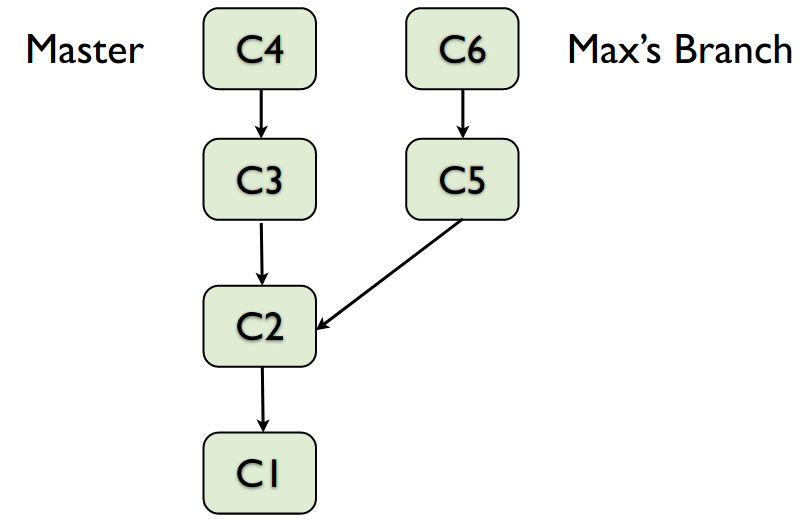
\includegraphics[scale=0.3]{branch2.png} \\ \\

Si crea con: \begin{verbatim}         git branch <nome branch> \end{verbatim}
Sposta l'HEAD sul branch specificato: \begin{verbatim}         git checkout testing\end{verbatim}
Sposta l'HEAD sul branch specificato e lo crea se non esiste:\begin{verbatim}         git checkout -b testing\end{verbatim}


\subsubsection{Merge}
Il merge è l'operazione di unione di due branch, "collassare i cambiamenti di un branch su un altro".
Prima di effettuare un merge, git fa un precheck per determinare se e come il merge può essere effettuato.

git log --all --oneline --merges dà una lista di tutti i commit che hanno fatto un merge.

Esistono due tipi di merge:
\paragraph{3-way merge}
Si verifica in caso di attività parallele, in cui il merge creerà un commit addizionale che effettua il merge dei due branch.
\paragraph{Fast-forward merge}
può essere effettuato quando viene fatto un branch che non devia mai dal branch master.\\ \\
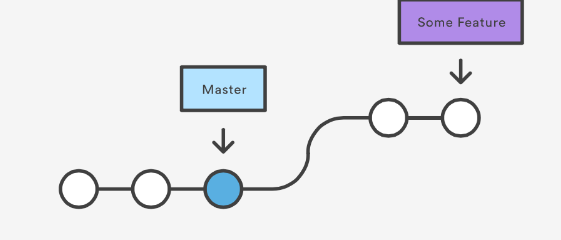
\includegraphics[scale=0.4]{mergeff.png} \\ \\

\subsubsection{Rebase}


\subsubsection{Branch implicito}
Si crea quando ci sono utenti che lavorano  in parallelo su repository locali diverse.

\subsubsection{Stashing and cleaning}
Supponiamo che sia a metà strada con il lavoro, ma si ha il bisogno di passare a qualcos'altro, per esempio un branch diverso.
Facendo stash si mettono da parte le modifiche che poi, si potranno riapplicare di nuovo anche in un branch diverso.

\subsubsection{Git reset}%vs checkout


\subsubsection{Pull request}
Informa altri del codice di un branch che è stato pushato in una repository, in modo tale da effettuare code review e eventualmente accettare e fare il merge del branch.

Pull Request Workflow\\
1. Developer creates a feature in a branch (locally)\\
2. The branch is pushed in the central repository\\
3. The developer fills and submits a pull request\\
4. The team reviews the code, discusses and modifies it\\
5. The project maintainer performs the merge and closes the pull request\\

Contributing to somebody else's project through a pull request
1. Fork the original repository, then clone it locally\\
2. Create a branch and contribute with your changes\\
3. Configure upstream fetch from the original repository (so you can update your repo with newer changes from there)\\
4. Fetch remote changes\\
5. Push your changes to your repo\\
6. Open a pull request\\

\chapter{Build Automation Scripts}
Tutte le dipendenze di un'applicazione vengono memorizzate nell'IDE e sono relative alla macchina che ospita tali configurazioni. Quando la stessa applicazione vuole essere rebuildata su un'altra macchina in molti casi non è semplice riprodurre l'ambiente originale, impedendo il rebuild.
Gli script di build risolvono tali problemi innanzitutto rendendo l'applicazione indipendente dall'IDE. Tuttavia le sue funziona vanno oltre: il build di script automatizza il processo di build, ma non solo la compilazione, fa anche operazioni di analisi statica automatica, testing, packaging, deploying, generazione di documentazione.
\section{Makefile}
Utility Unix che serve per automatizzare la build di un programma, nasce per automatizzare la compilazione, ma per come è fatto un makefile può automatizzare qualsiasi cosa: esso è un insieme di regole quindi, così come lancia la compilazione, può lanciare qualsiasi altra applicazione(e.g. compilazione latex).
L'idea base di Makefile è di creare dipendenze tra artefatti, come tra file .o e .c quando si compila programmi C.
Il makefile non è da confondere con un semplice script di shell, poiché quest'ultimo, ad ogni sua esecuzione, andrebbe a ricompilare tutto il programma, e ciò per un programma molto grande è overhead.
Invece il makefile va a controllare i timestamp delle dipendenze e degli artefatti: se il timestamp della dipendenza è più recente di quello dell'artefatto, questo verrà rigenerato, altrimenti tale operazione non sarà eseguita.
Un makefile contiene istruzione per creare file (gcc -c main.c) e le dipendenze tra i file.\\
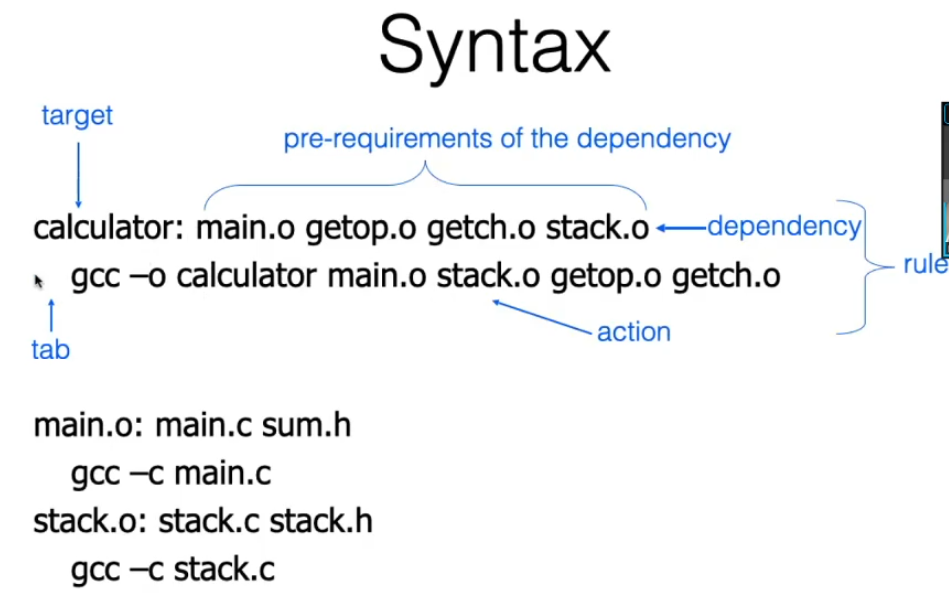
\includegraphics[scale=0.3]{makefile.png} \\
viene eseguito invocando il comando \textit{make} nella directory che contiene il Makefile.\\

\section{Apache Ant}
Concepito per JAva, eredita molti principi dal makefile ed è basato su XML, prevede una serie di task predefiniti utili per compilare, testare e così via.
A differenza di un makefile che ha comandi di shell, Ant ha dei task predefiniti invocati con dei tag XML.\\
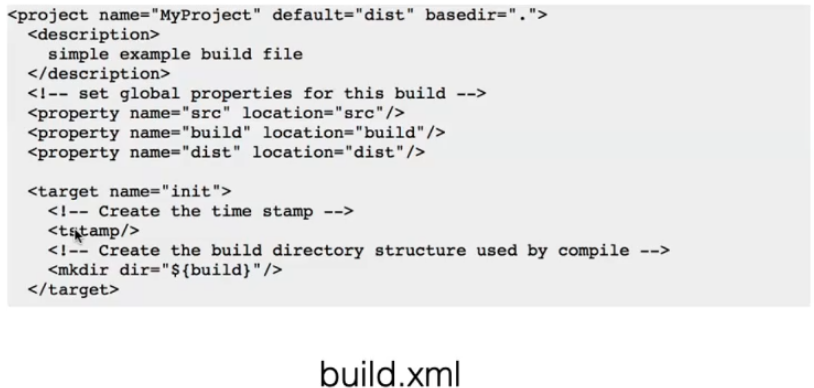
\includegraphics[scale=0.5]{ant.png} \\

\section{Apache Maven}
Strumento che aumenta il grado di automazione, rendendo tutto implicito (e.g. tutti i file in src sono da compilare, tutti quelli in test sono per eseguire i test).
Quindi non è richiesta la definizione di regole esplicite, ma bisogna organizzare la struttura del progetto in un certo modo predefinito. Tale struttura delle cartelle è nota a Maven quindi, se deve compilare o fare altre azion,i le farà senza bisogno di ulteriori configurazioni.
La peculiarità più importante di Maven è la gestione delle dipendenze. Infatti, Maven scarica automaticamente le dipendenze richieste dal suo repositor2y centrale o da altri repo.\\
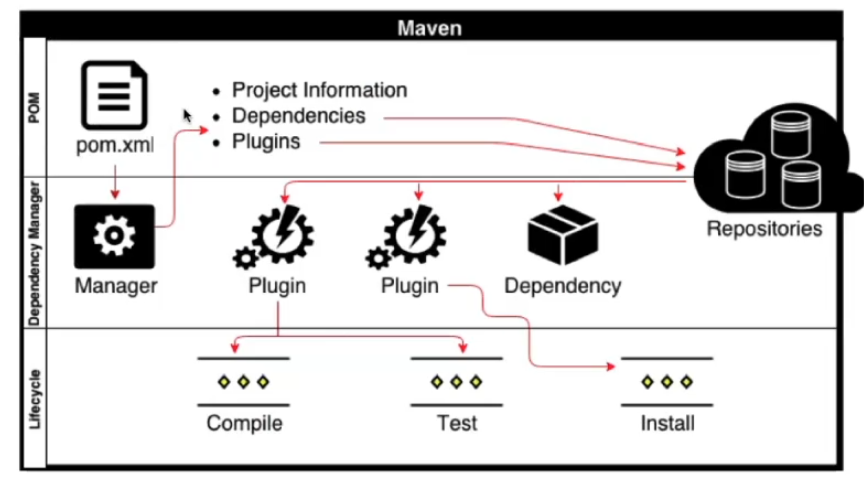
\includegraphics[scale=0.4]{maven.png} \\
Il file di build pom.xml viene interpretato dal manager che si assicura che le dipendenze e i plugins si trovino in locale altrimenti le recupera dal repo.
I plugin servono per eseguire dei task(e.g. compilazione java o altro linguaggio, svolgimento test...).


\section{Gradle}
sistema open source per l'automazione dello sviluppo fondato sulle idee di Apache Ant e Apache Maven, che introduce un domain-specific language (DSL) basato su Groovy, al posto della modalità XML usata da Apache Maven per dichiarare la configurazione del progetto. Gli script Gradle possono essere eseguiti direttamente, in contrasto con le definizioni dei progetti Apache Maven (pom.xml).\\
Gestisce le dipendenze come Maven (struttura progetto ecc).\\
Il file di build gradle si chiama \textbf{build.gradle} e al suo interno si trovano i \textbf{task} (attività)

\paragraph{Compilazione java}
nel file build.gradle: apply plugin: 'java'


\marginpar{videolezione 2021-10-15 pratica su gradle+info gruppi e progetto}






























\end{document}
